\documentclass{article}
\usepackage{url}
\usepackage{tabularx}
\usepackage{amssymb}
\usepackage{amsmath}
\usepackage[margin=1in]{geometry}
\usepackage[nottoc]{tocbibind}
\usepackage{graphicx}
\usepackage{adjustbox}
\usepackage{float}
\usepackage{changepage}
\graphicspath{ {./img/} }

\title{STAT UN2103 Homework 6}
\author{
  Jackson Chen
  \and
  jc4697
}
\date{\today}

\begin{document}
  \maketitle

  \section{Introduction}

    The purpose of this project is to conduct analysis on data containing a variety
    demographic factors regarding wages. More specifically, the aim is to determine
    a model with worker demographics as the covariates and the wage as a response variable.
    The model is supposed to correlate the input data as much as possible, so that the
    model would be able to be an effective predictive tool for wages. Creating a more
    realistic model also allows us to examine the larger research question surrounding
    this project, which is as follows:
    \begin{quote}
      Do African Americans have statistically different wages compared to Caucasian males?
      How do their wages also statistically compare all other males?
    \end{quote}

    The covariates included in the data consist of years of education (\texttt{edu} or $x_1$),
    job experience (\texttt{exp} or $x_2$), working in or near a city (\texttt{city} or $x_3$),
    US region (\texttt{reg} or $x_4$), race (\texttt{race} or $x_5$), college graduate
    (\texttt{deg} or $x_6$), and commuting distance (\texttt{com} or $x_7$). The data
    set also includes data for the response variable wages (\texttt{wage} or $Y$).

    In order to effectively train a model and test it, the input data was split into
    a training and a validation set. The input dataset initially had around $25,000$
    data points. The validation data set had 4965 entries, or about
    $20\%$ of the input dataset. The training set consisted of the remaining $80\%$ of
    the rows. A quality assurance check was then done on the split sets in order to assure
    relative heterogeneity of the datasets.

    Exploratory data analysis was conducted on the training dataset. The process will be
    described in the following sub-sections.

    \subsection{Preliminary Model Investigation}


  \section{Statistical Model} \label{final_model}

  \section{Research Question}

  \section{Appendix}
    This section contains the exact process that led to the determination of the final
    model described in Section \ref{final_model}. This process can be broken into two steps:
    The selection, transformation, and interaction of the covariates that created the
    final model, and the validation of the final model against a range of diagnostic tools.

    \subsection{Model Selection}
      The first step in the exploratory data analysis consisted of creating new columns in the
      data frame to map the categorical string variables \texttt{deg, city, reg, race} into
      numeric categorical variables. The purpose of this step is to satisfy the signature for \texttt{R}'s \texttt{I()}
      function, which groups covariates together into an interaction variable.

      After the training-validation split was done on the data, a QQ plot was plotted on
      the untransformed dataset, as shown in Figure \ref{fig:qqwage}. However the end
      of the QQ plot had too extreme of a vertical gradient. Therefore a logarithmic
      transformation would reduce the extremity at this end. Figure \ref{fig:qqlogwage}
      shows the QQ plot on the logarithmically transformed response variable. The
      overall structure of the points as well as the end behavior are much more
      normal.

      \begin{figure}
        \centering
        \begin{minipage}{.45\textwidth}
          \centering
          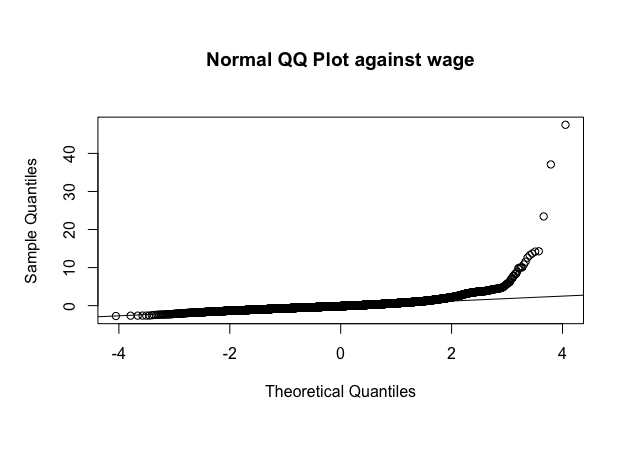
\includegraphics[scale=0.35]{transformation/qqwage}
          \caption{QQ plot on untransformed wage}
          \label{fig:qqwage}
        \end{minipage}
        \begin{minipage}{.45\textwidth}
          \centering
          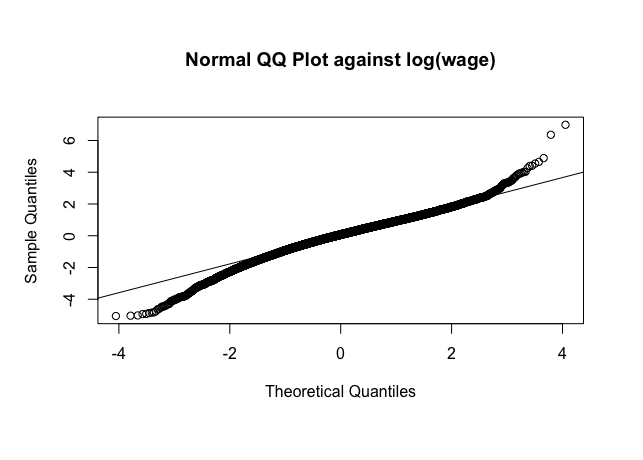
\includegraphics[scale=0.35]{transformation/qqlogwage}
          \caption{QQ plot on log transformed wage}
          \label{fig:qqlogwage}
        \end{minipage}
      \end{figure}

      The next step involved verifying whether each of the covariates in the input dataset
      actually correlated with \texttt{wage}. This purpose was this was to determine
      which variables to investigate further in terms of transformations, functional forms,
      and interactions. The more formal process for eliminating covariates occurs in the
      reduction of explanatory variables stage.

      From Figure \ref{fig:scattercom}, it appears that the commute time has no impact
      on wages. This is determined visually by examining that the linear smoothing of the graph
      has no gradient and thus indicates no relationship. We can verify this more numerically
      by running a marginal t-test on a linear model between the wages and the commute time.
      The null hypothesis in this test predict that $\beta_1 = 0$, with the commute time
      as the $x_1$ term. Running the t-test in \texttt{R} calculates the p value to be 0.79,
      which is greater than the 0.05 significance cutoff, indicating the failure to reject
      the null hypothesis. The following is the \texttt{R} output.

      \begin{verbatim}
        Call:
        lm(formula = log(data$wage) ~ data$com)

        Coefficients:
                     Estimate Std. Error t value Pr(>|t|)
        (Intercept) 6.2634186  0.0079812 784.770   <2e-16 ***
        data$com    0.0001497  0.0005631   0.266     0.79
        ---
        Signif. codes:  0 ‘***’ 0.001 ‘**’ 0.01 ‘*’ 0.05 ‘.’ 0.1 ‘ ’ 1

        Residual standard error: 0.6351 on 19856 degrees of freedom
        Multiple R-squared:  3.559e-06,	Adjusted R-squared:  -4.68e-05
        F-statistic: 0.07067 on 1 and 19856 DF,  p-value: 0.7904
      \end{verbatim}

      On the other hand, the other covariates show an existent relationship with wages
      (or the log of the wage). Figures \ref{fig:scatterexp} to \ref{fig:boxrace} provide
      graphical support behind such claims. Only a select number of covariates were displayed
      since the graphs behind the other covariates follow a very similar trend. By
      observing the smoothing functions for all of the aforementioned graphs,
      one can determine the transformations necessary to construct the
      most predictive linear model with respect to wages. Most of the smoothing
      functions indicate a somewhat linear path indicating a strict linear relationship,
      with one exception.

      Figure \ref{fig:scatterexp} depicts a downward-facing
      quadratic relationship between the number of years of experience and the log
      of the wages. Upon further inspection, Figure \ref{fig:boxexp} represents
      the relationship more clearly with the inner quartile ranges following the
      same quadratic trend. Therefore, \texttt{exp} requires a quadratic transformation
      to resolve this violation in linearity. \\

      \begin{figure}
        \centering
        \begin{minipage}{.45\textwidth}
          \centering
          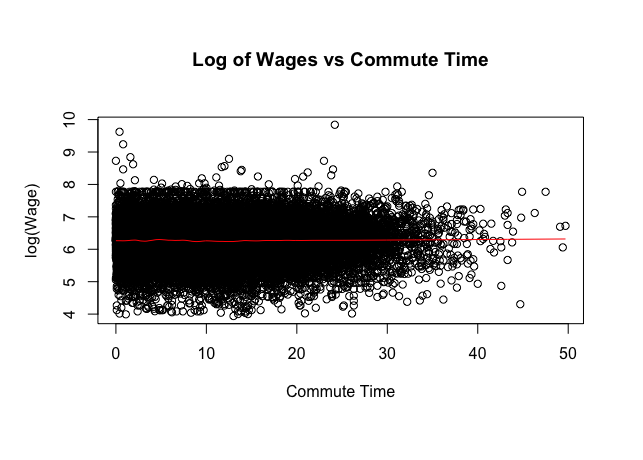
\includegraphics[scale=0.35]{transformation/scattercom}
          \caption{Scatter plot on commute time}
          \label{fig:scattercom}

          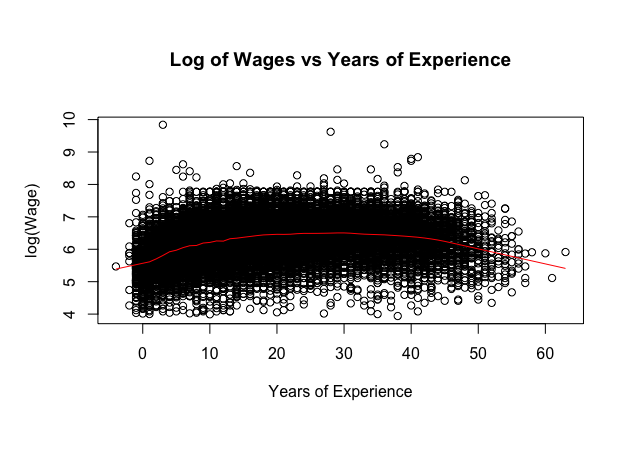
\includegraphics[scale=0.35]{transformation/scatterexp}
          \caption{Scatter plot on years of experience}
          \label{fig:scatterexp}

          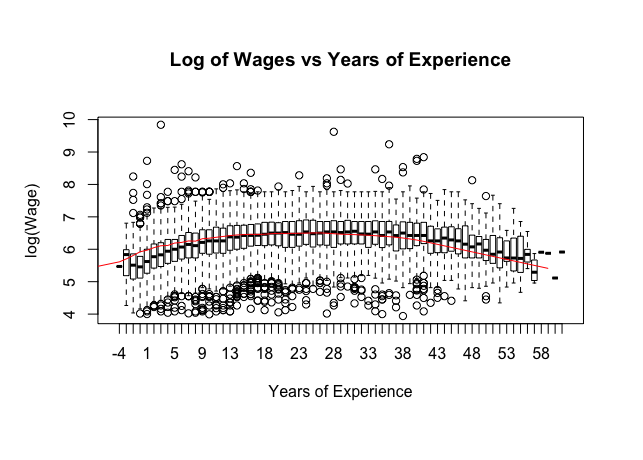
\includegraphics[scale=0.35]{transformation/boxexp}
          \caption{Box plot on years of experience}
          \label{fig:boxexp}
        \end{minipage}
        \begin{minipage}{.45\textwidth}
          \centering
          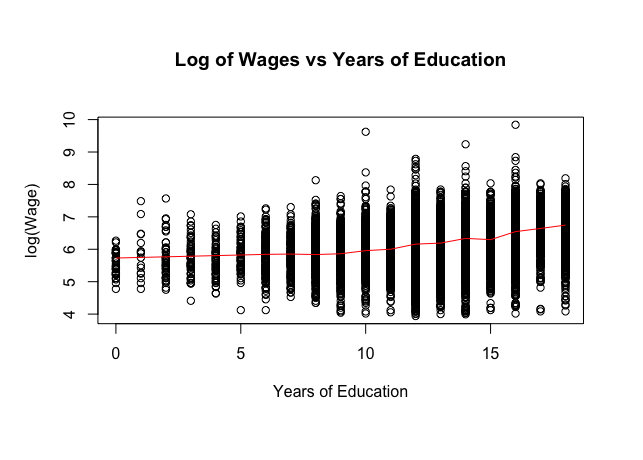
\includegraphics[scale=0.35]{transformation/scatteredu}
          \caption{Scatter plot on number of employees}
          \label{fig:scatteredu}

          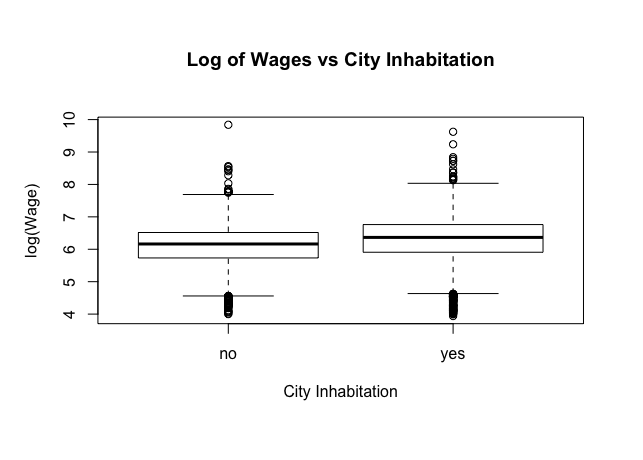
\includegraphics[scale=0.35]{transformation/boxcity}
          \caption{Scatter plot on number of employees}
          \label{fig:boxcity}

          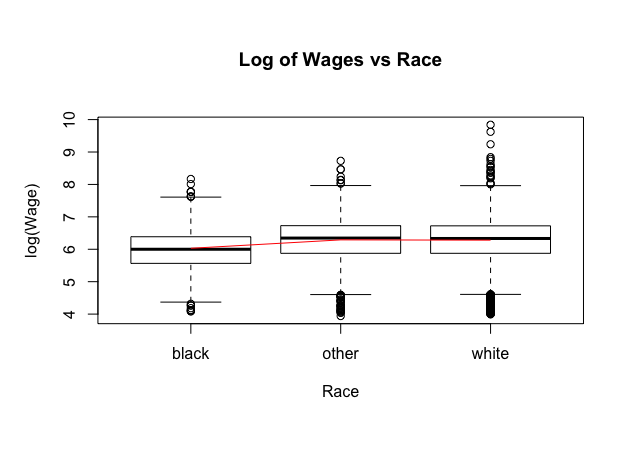
\includegraphics[scale=0.35]{transformation/boxrace}
          \caption{Scatter plot on number of employees}
          \label{fig:boxrace}
        \end{minipage}
      \end{figure}

      At this stage of the analysis, we have determined that the model will have
      a logarithmically transformed response variable \texttt{wage}, a quadratically
      transformed covariate \texttt{exp}, and linear relationships for all other covariates.
      Mathematically speaking, the equation is:
      \[ \log{Y} = \beta_0 + \beta_1 x_1 + \beta_2 x_2 + \beta_3 x_2^2 + \beta_4 x_3
                     + \beta_5 x_4 + \beta_6 x_5 + \beta_7 x_6 + \beta_8 x_7\]


      The last important component of the model now needs to be examined:
      interactions between covariates. This analysis will consist of three parts:
      \begin{enumerate}
        \item Interactions among categorical variables
        \item Interactions between categorical and continuous variables
        \item Interactions among continuous variables
      \end{enumerate}

      Testing for collinearity among categorical variables requires testing every
      pair of two variables. Since there are 4 categorical variables, this results
      in 6 tests. Each test consists of generating an interaction graph between the
      two chosen variables and the response variable $log(\text{Wage})$. These graphs
      are displayed in Figures \ref{fig:interactionregioncity} to
      \ref{fig:interactiondegreerace}. Each test also consists of running a
      Type I Sum of Squares ANOVA test to numerically check for multilinearity.

      Region and city are correlated. Figure \ref{fig:interactionregioncity} show
      that the lines for each region intersect, indicating that the worker's region
      influences the rate at which living in a city increases ones wages. Numerically,
      we can use a marginal t-test to ensure that a correlation between \texttt{reg}
      and \texttt{city} is statistically significant.

      The null hypothesis in this situation states that there exists no relationship
      between region and city. The alternate hypothesis states the contrary. Using
      \texttt{R}, we compute the p value to be 0.0021 which is less than the required
      0.05 significance. Therefore we reject the null hypothesis and accept $H_A$,
      which states that a statistically significant relationship between region and
      city exists. The following is the sample \texttt{R} output. Note how the
      final variable is combined into an interaction variable, allowing the marginal
      t-test to be run.

      \begin{verbatim}
        Call:
        lm(formula = log(data$wage) ~ city + reg + I(city_num * reg_num),
            data = data)

        Coefficients:
                              Estimate Std. Error t value Pr(>|t|)
        (Intercept)            6.01866    0.04720 127.515  < 2e-16 ***
        cityyes                0.27351    0.02907   9.409  < 2e-16 ***
        regnortheast           0.07304    0.01695   4.309 1.65e-05 ***
        regsouth              -0.16686    0.01797  -9.284  < 2e-16 ***
        regwest               -0.10474    0.02949  -3.552 0.000383 ***
        I(city_num * reg_num)  0.03174    0.01030   3.082 0.002057 **
        ---
        Signif. codes:  0 ‘***’ 0.001 ‘**’ 0.01 ‘*’ 0.05 ‘.’ 0.1 ‘ ’ 1

        Residual standard error: 0.6256 on 19852 degrees of freedom
        Multiple R-squared:   0.03,	Adjusted R-squared:  0.02976
        F-statistic: 122.8 on 5 and 19852 DF,  p-value: < 2.2e-16
      \end{verbatim}

      According to Figure \ref{fig:interationdegreecity}, city and degree
      are also correlated. The slopes, although less noticeable compared
      to the previous case, are different. To verify this numerically, an
      ANOVA test will be run between city and degree, and wages. In this
      situation, we will examine the SSR values to determine correlation
      rather than the marginal t-test.

      We will run the ANOVA test with \texttt{city} as $x_1$ and \texttt{deg} as $x_2$,
      and then another ANOVA test with \texttt{city} as $x_2$ and \texttt{deg} as $x_1$.
      These are the respective \texttt{R} outputs.

      \begin{verbatim}
        Analysis of Variance Table

        Response: log(data$wage)
                     Df Sum Sq Mean Sq F value    Pr(>F)
        data$city     1  153.9  153.91  414.42 < 2.2e-16 ***
        data$deg      1  481.9  481.89 1297.52 < 2.2e-16 ***
        Residuals 19855 7374.0    0.37
        ---
        Signif. codes:  0 ‘***’ 0.001 ‘**’ 0.01 ‘*’ 0.05 ‘.’ 0.1 ‘ ’ 1
      \end{verbatim}

      \begin{verbatim}
        Analysis of Variance Table

        Response: log(data$wage)
                     Df Sum Sq Mean Sq F value    Pr(>F)
        data$deg      1  521.0  520.96 1402.74 < 2.2e-16 ***
        data$city     1  114.8  114.84  309.21 < 2.2e-16 ***
        Residuals 19855 7374.0    0.37
        ---
        Signif. codes:  0 ‘***’ 0.001 ‘**’ 0.01 ‘*’ 0.05 ‘.’ 0.1 ‘ ’ 1
      \end{verbatim}

      If the two variables are perfectfully uncorrelated, then the following two
      statements are true:
      \begin{align*}
        SSR(x_1 | x_2) &= SSR(x_1) \\
        SSR(x_2 | x_1) &= SSR(x_2)
      \end{align*}

      However, from the above \texttt{R} output, the sum of squares values in the
      ANOVA table change significantly for both \texttt{city} and \texttt{deg}
      between the two commutative models. For example, assuming that \texttt{city} is $x_1$,
      $SSR(x_1) = 153.9$ while $SSR(x_1 | x_2) = 114.8 \implies SSR(x_1) \neq SSR(x_1 | x_2)$.
      Therefore \texttt{deg} and \texttt{city} are correlated.

      Both the SSR method and marginal t-test method are rigorous methods to
      verify statistical significance between two variables. Future examples
      will use the marginal t-test for the sake of simplicity. Furthermore,
      future correlations will not go as in depth as the previous two cases
      because the process is algorithmically the same.

      The final correlated case between two categorical variables is between
      region and degree, since Figure \ref{fig:interactionregiondegree} demonstrates
      that the degree slopes are different per region. The p value from the
      t-test is 0.0031, rejecting the null hypothesis and accepting the alternate
      hypothesis that region and degree are related.
      On the other hand, the other three pairings:
      \texttt{city} vs \texttt{race}, \texttt{region} vs \texttt{race}, and
      \texttt{degree} vs \texttt{race} show no interaction because the results
      from their marginal t-tests failed to reject the null hypotheses. \\

      \begin{figure}
        \centering
        \begin{minipage}{.45\textwidth}
          \centering
          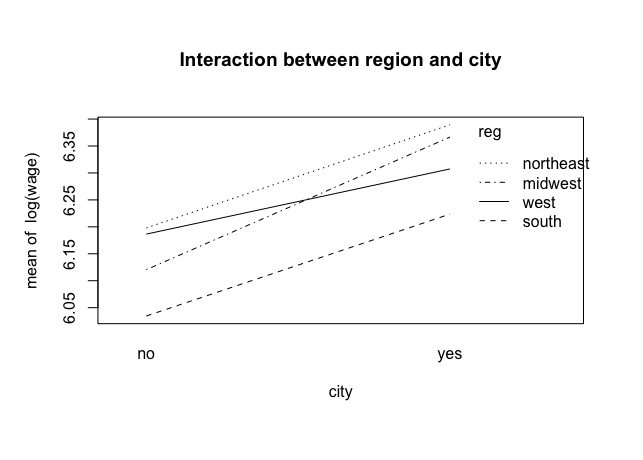
\includegraphics[scale=0.35]{interaction/regioncity}
          \caption{Regional influence on city's relationship with wage}
          \label{fig:interactionregioncity}

          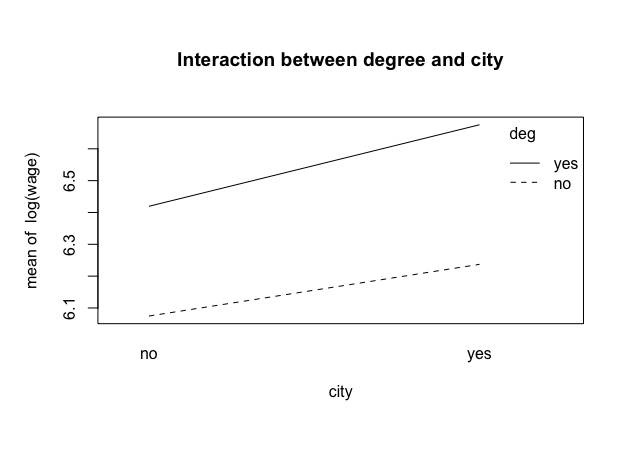
\includegraphics[scale=0.35]{interaction/degreecity}
          \caption{College degree's influence on city's relationship with wage}
          \label{fig:interationdegreecity}

          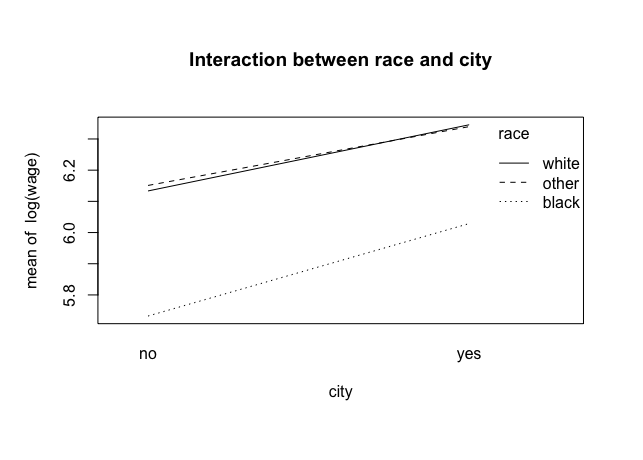
\includegraphics[scale=0.35]{interaction/racecity}
          \caption{Racial influence on city's relationship with wage}
          \label{fig:interactionracecity}
        \end{minipage}
        \begin{minipage}{.45\textwidth}
          \centering
          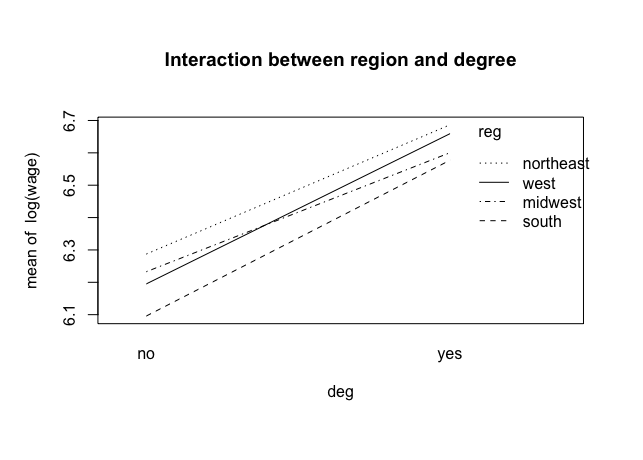
\includegraphics[scale=0.35]{interaction/degreeregion}
          \caption{Regional influence on degree's relationship with wage}
          \label{fig:interactionregiondegree}

          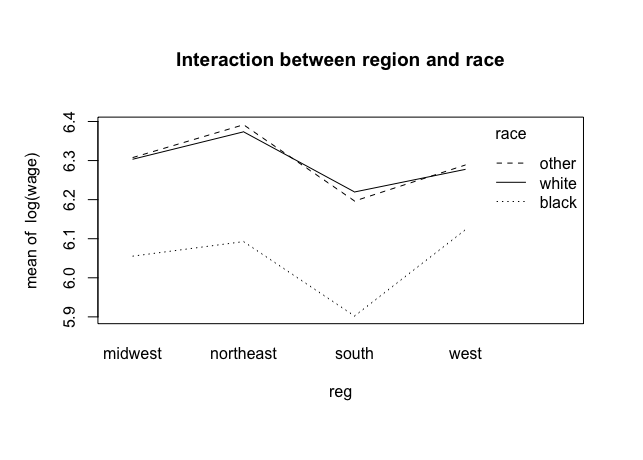
\includegraphics[scale=0.35]{interaction/regionrace}
          \caption{Racial influence on region's relationship with wage}
          \label{fig:interactionregionrace}

          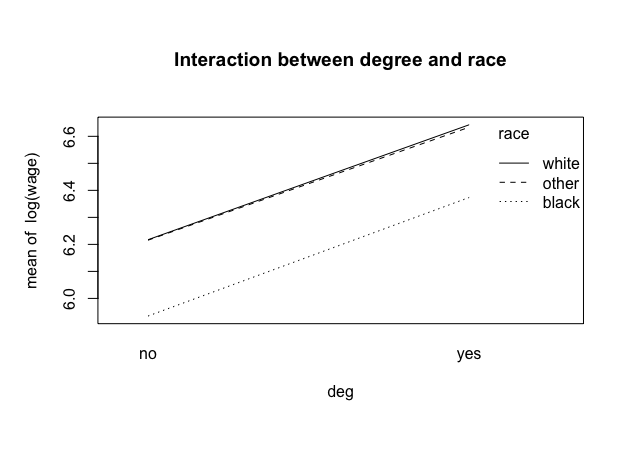
\includegraphics[scale=0.35]{interaction/degreerace}
          \caption{Racial influence on degree's relationship with wage}
          \label{fig:interactiondegreerace}
        \end{minipage}
      \end{figure}

      The next batch of interactions to check for is between categorical and
      continuous variables. Only the graphs of correlated variables will
      be shown (Figures \ref{fig:interactionedurace} to \ref{fig:interactionregedu}).
      Uncorrelated variables have graphs with slopes that do not change between
      different the categories, and have p values greater than 0.05 when running
      the marginal t-test.

      The graphs of the collinear variables all contain regression lines that
      intersect, indicating that the slopes are influenced by the categorical
      variable. We will run the marginal t-test on all of these pairs of variables
      to ensure that their relationship is statistically significant. The null
      hypotheses for each of these pair of tests state that the relationship
      between the two given variables is not statistically significant. All of the
      respective p-values for these t-tests are shown in Table \ref{tab:p-val}.

      \begin{table}[H]
        \centering
        \begin{tabular}{lll}
        \textbf{Categorical} & \textbf{Continuous} & \textbf{p-value} \\
        Race                 & Education           & 0.0171           \\
        Race                 & Experience          & 0.00177          \\
        City                 & Experience          & 0.0219           \\
        Degree               & Education           & 3.35e-05         \\
        Degree               & Experience          & 5.14e-09         \\
        Region               & Education           & 0.00571
        \end{tabular}
        \caption{p values for correlated categorical and continuous variables.}
        \label{tab:p-val}
      \end{table}

      Since every p value in this table is less than 0.05 significance, the
      null hypothesis would be rejected in every associated marginal t-test.
      Therefore the alternate hypothesis is accepted. $H_A$ states that the
      variables are statistically related. Therefore we must include interactions
      between these variables in our final model to predict wages.

      One can verify that these correlated variables are practical in the context of the real world.
      The relationships between degree and education and between degree and
      experience are very strongly correlated due to the very small p value.
      This makes sense since a certain amount of years of education directly leads
      to a degree, and having a degree can guarantee job experience. \\

      \begin{figure}
        \centering
        \begin{minipage}{.45\textwidth}
          \centering
          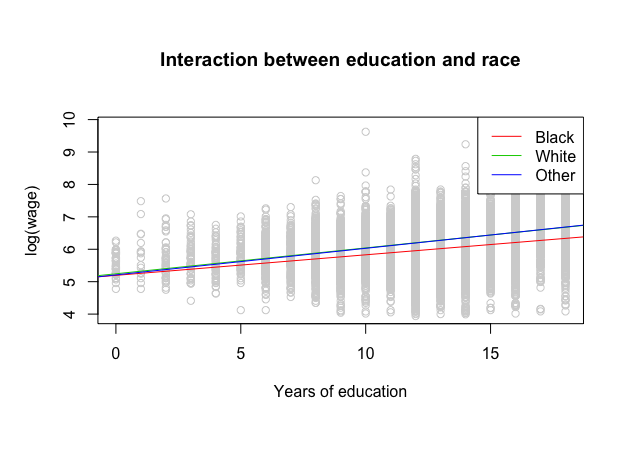
\includegraphics[scale=0.35]{interaction/edurace}
          \caption{Racial influence on education's relationship with wage}
          \label{fig:interactionedurace}

          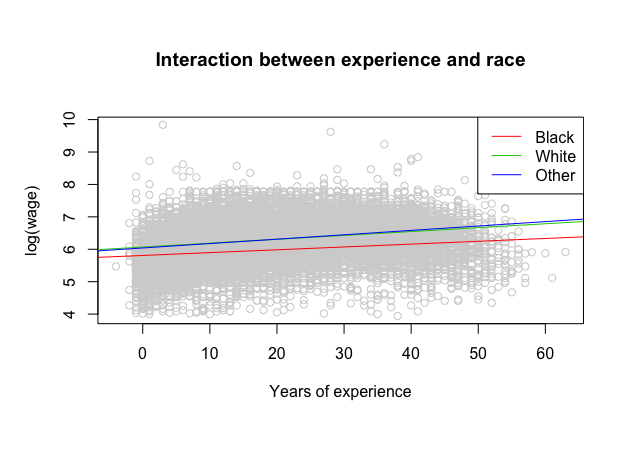
\includegraphics[scale=0.35]{interaction/exprace}
          \caption{Racial influence on experience's relationship with wage}
          \label{fig:interationexprace}

          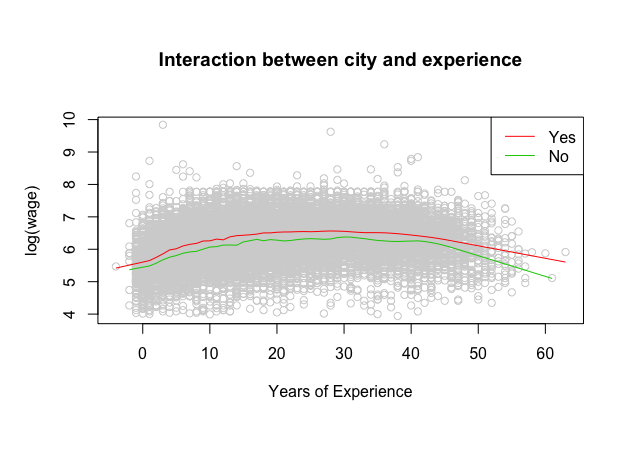
\includegraphics[scale=0.35]{interaction/cityexp}
          \caption{City influence on experience's relationship with wage}
          \label{fig:interactioncityexp}
        \end{minipage}
        \begin{minipage}{.45\textwidth}
          \centering
          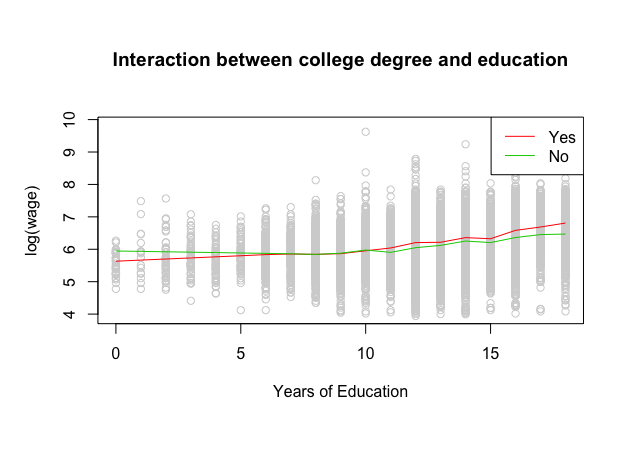
\includegraphics[scale=0.35]{interaction/degedu}
          \caption{Degree influence on education's relationship with wage}
          \label{fig:interactiondegedu}

          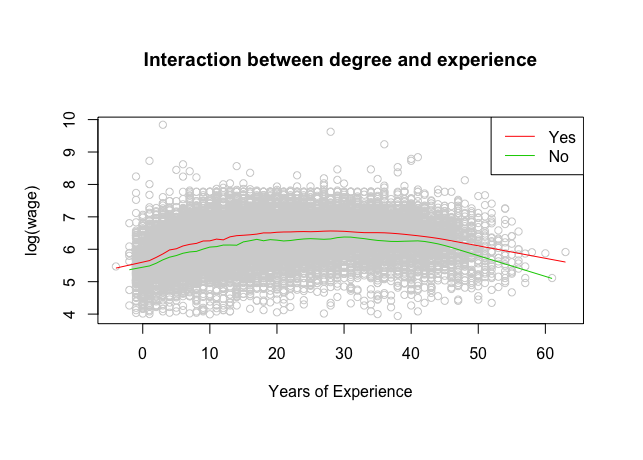
\includegraphics[scale=0.35]{interaction/degexp}
          \caption{Degree influence on experience's relationship with wage}
          \label{fig:interactioncdegexp}

          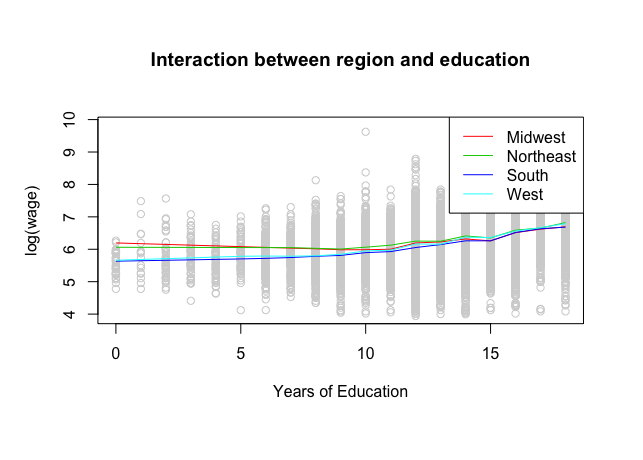
\includegraphics[scale=0.35]{interaction/regedu}
          \caption{Regional influence on education's relationship with wage}
          \label{fig:interactionregedu}
        \end{minipage}
      \end{figure}

      The last category of correlated variables consist of correlated continuous
      variables. To determine which continuous variables are correlated,
      use \texttt{R} to populate a correlation table between the covariates
      in question. Table \ref{tab:correlated} contains the correlation coefficients
      between each pair of continuous variable.

      \begin{table}[H]
        \centering
        \begin{tabular}{lllllll}
                        &  \textbf{log(wage)}   &    \textbf{education}  &  \textbf{experience}   & \textbf{$(\text{experience})^2$} & \textbf{commute}       & \textbf{employees} \\
        \textbf{log(wage)}       &  1.000000000 &  3.697235e-01 &  2.327511e-01 & -2.920242e-01 & 1.886612e-03  &  0.059898053 \\
        \textbf{education}       &  0.369723477 &  1.000000e+00 & -2.793636e-01 & -1.530700e-01 & -2.564785e-05 &   0.020344053 \\
        \textbf{experience}      &  0.232751149 & -2.793636e-01 &  1.000000e+00 &  5.146722e-16 & 7.603960e-03  & -0.003872245 \\
        \textbf{$(\text{experience})^2$}  & -0.292024228 & -1.530700e-01 &  5.146722e-16 &  1.000000e+00 & -4.578743e-03 &  -0.017773812 \\
        \textbf{commute}         &  0.001886612 & -2.564785e-05 &  7.603960e-03 & -4.578743e-03 & 1.000000e+00  & -0.003173171 \\
        \textbf{employees}       &  0.059898053 &  2.034405e-02 & -3.872245e-03 & -1.777381e-02 & -3.173171e-03 &   1.000000000
        \end{tabular}
        \caption{Correlation coefficients between every pair of continuous variable.}
        \label{tab:correlated}
      \end{table}

      In the correlation table, only correlation values above 0.05 or below -0.05
      will be considered correlated. Only one pair of continuous variables satisfies
      this requirement: education and experience. We can verify that this is the
      case by running a marginal t-test. The null hypothesis states that education
      and experience are not statistically correlated. The p value calculated by \texttt{R}
      is $2 * 10^{-6}$, which is less than the 0.05 significance threshold. Therefore
      we reject the null hypothesis and accept that \texttt{edu} and \texttt{exp} are
      statistically related. \\

      At this stage, we have discovered all of the interactions between the covariates
      as well as any transformations that are needed to satisfy linearity. The
      mathematical model at this state can be summed up with:

      \begin{align*}
        \log{Y} = &\beta_0 + \beta_1 x_1 + \beta_2 x_2 + \beta_3 x_2^2 + \beta_4 x_3 \\
                    &+ \beta_5 x_4 + \beta_6 x_5 + \beta_7 x_6 + \beta_8 x_7 \\
                    &+ \beta_9 x_1 x_2 \\
                    &+ \beta_{10} x_1 x_5 + \beta_{11} x_2 x_5 + \beta_{12} x_1 x_6 + \beta_{13} x_2 x_6 + \beta_{14} x_1 x_4 + \beta_{15} x_2 x_3 \\
                    &+ \beta_{16} x_3 x_4 + \beta_{17} x_3 x_6 + \beta_{18} x_4 x_6
      \end{align*}

      Now that the preliminary model investigation is complete and that all of the
      functional forms and interactions have been included in the model, we now
      need to reduce the number of explanatory variables. In this study, we will
      use the best subsets procedure and optimize for Mallows' $C_p$.

      \begin{figure}
        \centering
        \begin{minipage}{.45\textwidth}
          \centering
          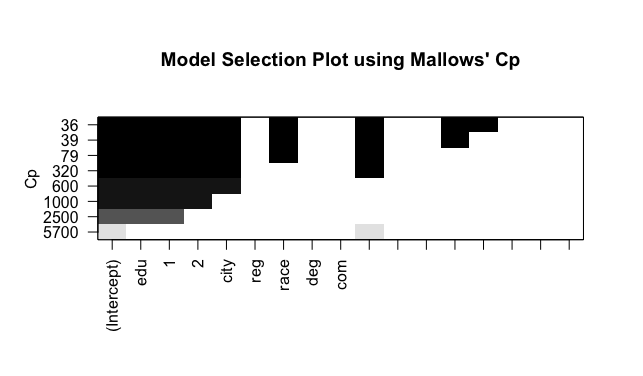
\includegraphics[scale=0.35]{selection/modelselect1}
          \caption{Model Selection Plot using Mallows' $C_p$}
          \label{fig:modelselect1}
        \end{minipage}
        \begin{minipage}{.45\textwidth}
          \centering
          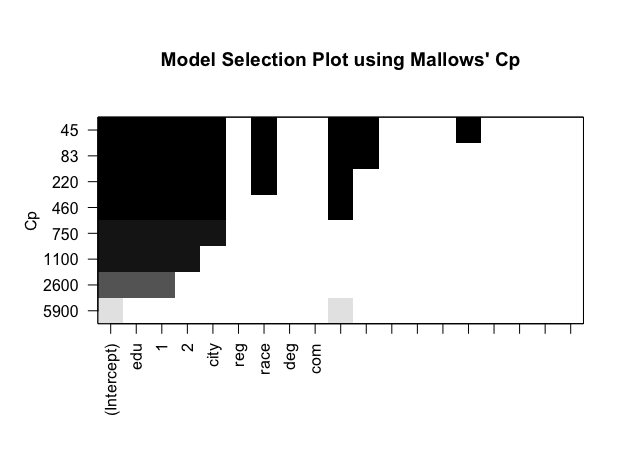
\includegraphics[scale=0.35]{selection/modelselect2}
          \caption{Model Selection Plot using Mallows' $C_p$ excluding the last term}
          \label{fig:modelselect2}
        \end{minipage}
      \end{figure}

      After using the \texttt{leap} library to generate model selection plots
      (Figures \ref{fig:modelselect1} and \ref{fig:modelselect2}) the final two models
      to pick from are:

      \begin{align}
        \log{Y} &= \beta_0 + \beta_1 x_1 + \beta_2 x_2 + \beta_3 x_2^2 + \beta_4 x_3 + \beta_5 x_5 + \beta_6 x_1 x_2 + \beta_7 x_1 x_5 + \beta_8 x_3 x_6 + \beta_9 x_4 x_6 \\
        \log{Y} &= \beta_0 + \beta_1 x_1 + \beta_2 x_2 + \beta_3 x_2^2 + \beta_4 x_3 + \beta_5 x_5 + \beta_6 x_1 x_2 + \beta_7 x_1 x_5 + \beta_8 x_1 x_4
      \end{align}

      AIC, $C_p$, $R^2$, and $R_a^2$ are three important criteria for model selection.
      Since Mallows' $C_p$ was used to generate these two models, we will not be
      using that criterion to compare the two models. Instead, the comparison will
      lie in the remaining 3 factors: AIC, $R^2$, $R_a^2$. The follow table contains
      these values for each model.

      \begin{table}[]
        \centering
        \begin{tabular}{lll}
            & \textbf{Model 1}  & \textbf{Model 2}  \\
        \textbf{AIC} & 29832.34 & 29844.68 \\
        \textbf{$R^2$}  & 0.3487   & 0.3487   \\
        \textbf{$R_a^2$} & 0.3482   & 0.3482
        \end{tabular}
        \caption{AIC, $R^2$, and $R_a^2$ scores for each model}
        \label{tab:selection}
      \end{table}

      As seen from Table \ref{tab:selection}, it appears that Model 1 has a
      slight edge over Model 2, since its AIC, $R^2$, and $R_a^2$ scores are
      consistently lower than that of Model 2's. Therefore Model 1 will be chosen
      as the final model for the dataset due to its slightly higher accuracy
      in its predictive power over Model 2.

    \subsection{Diagnostics and Model Validation}
      Since the final model has been chosen, the final step is to run
      diagnostics to validate the model's stability and reasonableness.

      We will conduct residual diagnostics to ensure that the linearity of
      the response function, the normality of the errors, and homoscedasticity
      are all maintained. The diagnostic plots are in Figures \ref{fig:histm1}
      to \ref{fig:scatterm1}.

      \begin{figure}[H]
        \centering
        \begin{minipage}{.45\textwidth}
          \centering
          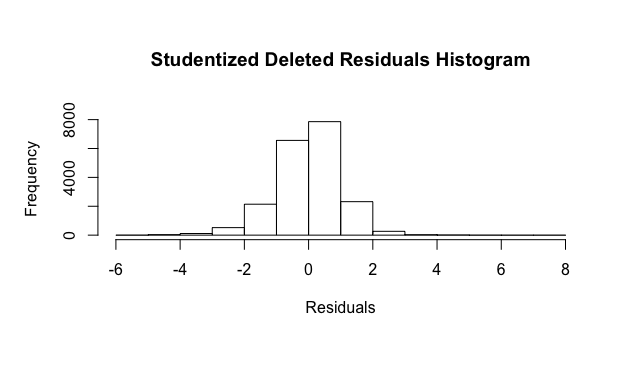
\includegraphics[scale=0.35]{selection/histm1}
          \caption{Studentized Deleted Residual Histogram for Model 1}
          \label{fig:histm1}

          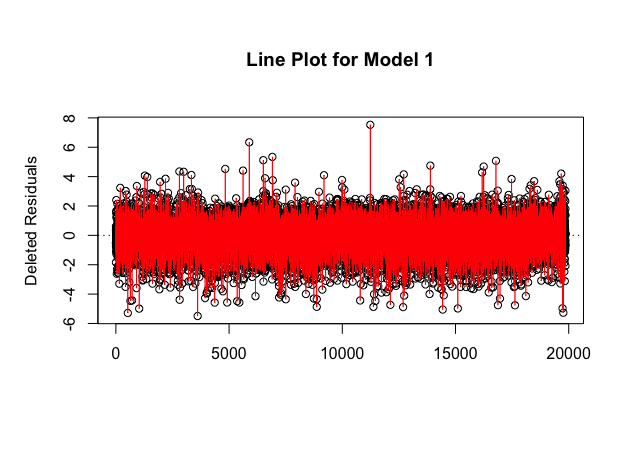
\includegraphics[scale=0.35]{selection/linem1}
          \caption{Studentized Deleted Residual Line Plot for Model 1}
          \label{fig:linem1}
        \end{minipage}
        \begin{minipage}{.45\textwidth}
          \centering
          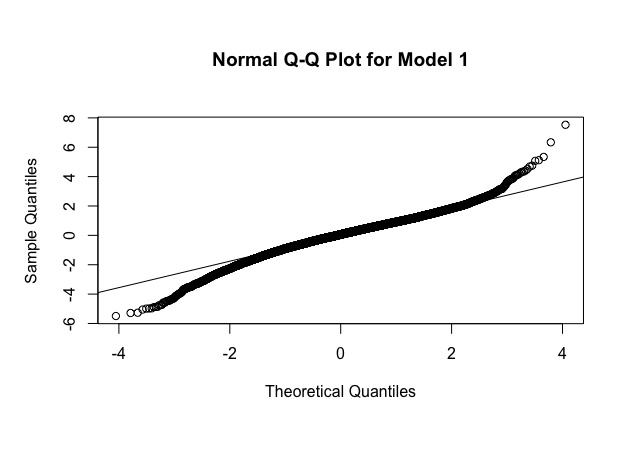
\includegraphics[scale=0.35]{selection/qqm1}
          \caption{Studentized Deleted Residual QQ Plot for Model 1}
          \label{fig:qqm1}

          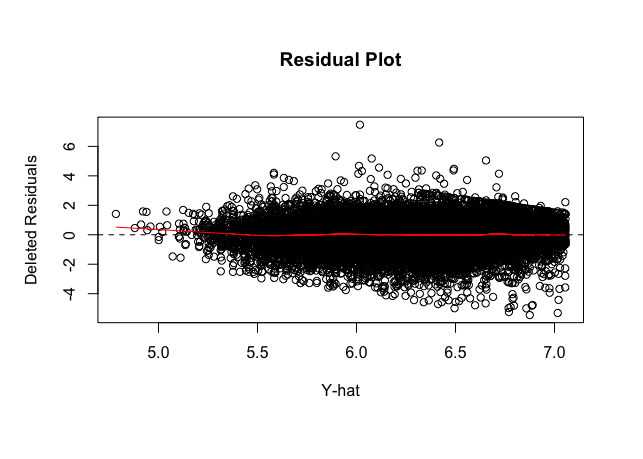
\includegraphics[scale=0.35]{selection/scatterm1}
          \caption{Studentized Deleted Residual Scatter Plot for Model 1}
          \label{fig:scatterm1}
        \end{minipage}
      \end{figure}

      Figure \ref{fig:histm1} indicates a histogram with a relatively normal
      distribution with a very small right skew. The QQ plot in Figure
      \ref{fig:qqm1} has slightly odd end behavior but is otherwise normal.
      The Line Plot in Figure \ref{fig:linem1} is seemingly random without
      much extreme outliars, as it is supposed to be. And finally, the
      residual plot in Figure \ref{fig:scatterm1} has a linear, zero gradient
      smoothing function, which is correct. In all, normality may be slightly
      skewed but the other properties related to linear regression models are
      satisfied. \\

      For model validation, we need to run the model on the unseen test dataset and
      measure the mean square prediction error. The relative proximity of MSPE with
      the mean square error will indicate how well the model responds to new data,
      and how strong its predictive capabilities are.

      According to \texttt{R}, the values are as follows:

      \begin{align*}
        MSE &= 0.2624992 \\
        MSPE &= 0.2623269
      \end{align*}

      These values are very closely aligned, indicating that our regression function
      is plausible, and has the ability to generalize inferences well.
\end{document}
